\documentclass[letterpaper, 11 pt, conference]{ieeeconf}  

\overrideIEEEmargins

\usepackage{graphics} % for pdf, bitmapped graphics files
\usepackage{epsfig} % for postscript graphics files

\usepackage{amsmath} % assumes amsmath package installed
\usepackage{amssymb}  % assumes amsmath package installed

\usepackage[ruled, vlined, linesnumbered]{algorithm2e}
%\usepackage{algorithm}
\usepackage{verbatim} 
%\usepackage[noend]{algpseudocode}
\usepackage{soul, color}
\usepackage{lmodern}
\usepackage{fancyhdr}
\usepackage[utf8]{inputenc}
\usepackage{fourier} 
\usepackage{array}
\usepackage{makecell}

%should help with urls for citations
\usepackage{url}

\usepackage{hyperref}

\usepackage{blindtext}
\usepackage{multicol}
\usepackage{lipsum}
\usepackage{float}
\usepackage[backend=biber]{biblatex}
\addbibresource{HIV.bib}



\SetNlSty{large}{}{:}

\renewcommand\theadalign{bc}
\renewcommand\theadfont{\bfseries}
\renewcommand\theadgape{\Gape[4pt]}
\renewcommand\cellgape{\Gape[4pt]}

\newcommand{\rework}[1]{\todo[color=yellow,inline]{#1}}

\makeatletter
\newcommand{\rom}[1]{\romannumeral #1}
\newcommand{\Rom}[1]{\expandafter\@slowromancap\romannumeral #1@}
\makeatother

\pagestyle{plain} 

\title{\LARGE \bf
Modeling the Within-Host Dynamics of HIV-1 Infection}

\author{Lily A. Crow% <-this % stops a space 
\\ Institute for Computing in Research \\
Portland, Oregon \\
lilyacrow@gmail.com\\}

\begin{document}

\maketitle
\thispagestyle{plain}
\pagestyle{plain}


%%%%%%%%%%%%%%%%%%%%%%%%%%%%%%%%%%%%%%%%%%%%%%%%%%%%%%%%%%%%%%%%%%%%%%%%%%%%%%%%
\begin{abstract}
%%%TODO:
Human Immunodeficiency Virus, commonly known as HIV, is the virus responsible for AIDS. HIV came front and center in the 1980's, as politics and 'religious beliefs' prevented patients from seeking testing, treatment, and support. Having three unique stages, it is in HIV's final stage, AIDS, that the immune system is no longer effective; a person can typically live for 3 years after having reached the threshold for AIDS. HIV targets CD4$^{+}$ T-cells, cells responsible for the immune response. Over the course of 10 years HIV destroys the CD4$^{+}$ count rendering the body unable to defend itself from opportunistic infections and malignancies. Over 40.4 million people have died from AIDS and nearly 86 million have tested positive for HIV, since its discovery in 1981 \cite{WHO, UNaids}. An important part of managing such a destructive epidemic is being able to effectively model the disease behaviors. Since the '90's, great strides have been made in mathematical modeling, in part due to advances in \emph{in vivo} modeling of HIV. Many models explore mutations in HIV viral genetics, latently infected cells, and the effects of combination antiretroviral therapy. This paper aims to demonstrate the within-host dynamics of HIV, with an emphasis on immune response and the effects of antiretroviral treatment. 

\end{abstract}
\begin{keywords}

CD4$^{+}$ T-cells, steady-state, viral load, antiretroviral therapy

\end{keywords}

%%%%%%%%%%%%%%%%%%%%%%%%%%%%%%%%%%%%%%%%%%%%%%%%%%%%%%%%%%%%%%%%%%%%%%%%%%%%%%%%
\section{INTRODUCTION TO HIV AND MATHEMATICAL MODELING}

Acquired Immunodeficiency Syndrome, also known as AIDS, was recognized as a new disease in 1981 after an increasing number of homosexual men died from unusual, and in many cases, rare, infections and malignancies- notably \emph{pneumocystis pneumonia} and \emph{Kaposi Sarcoma} \cite{OriginsofPandemic, LookBack, Fauci}. Patient's health declined in a rapid downward spiral as doctors struggled to treat one infection after another. It didn't take long for Human Immunodeficiency Virus to be identified as the cause of AIDS \cite{OriginsofPandemic}. At least 85.6 million people have been infected by HIV over the last 4 decades and 40.4 million have died \cite{WHO}. The first documented case of AIDS in the U.S. was in a homosexual male, and thus the public labeled AIDS as "'the gay plague'" \cite{LookBack}. Due to its prevalence in the LGBT+ community and among intravenous drug users, the public blamed AIDS on perceived lifestyle choices and moral 'flaws'. Not long after its discovery in the U.S., AIDS began to pop up in Haiti fueling rumors that it originated there \cite{LookBack}. Developing countries, particularly those in sub-Saharan Africa, have experienced the worst morbidity and mortality rates, with two thirds of living HIV positive patients residing in the WHO African Region \cite{WHO}. Similar to SARS in 2005, H1N1 in 2010, Ebola in 2015, and COVID-19 in 2020, the AIDS pandemic only fueled prejudice surrounding already marginalized groups, and stigma surrounding HIV grew worse \cite{RacialDiscrimination}. 

This growing stigma penetrated the highest places in the U.S. government. Then President Ronald Reagan and many of his senior officials, partook in the belief that homosexuals and drug users brought HIV/AIDS upon themselves by "engaging in immoral conduct". Reagan and his staff thought people infected by HIV were in greater need of moral reform than health policies, treatments, or resources \cite{Koop}. The Reagan administration withheld \$86 million dollars from the WHO, strangling its global HIV initiatives \cite{jhu}. The Surgeon General was sidelined and censured to prevent him from speaking to the public about HIV \cite{Koop}. Reagan refused to publicly mentioned AIDS until 1985, 4 years after the disease's discovery \cite{GSU}. It took him another 2 years (1987) for him to make a public speech on the matter \cite{GSU}. In the time between the discovery of AIDS and the President's delayed acknowledgement of the disease (1981-1987), 47,993 Americans died, nearly 1,000 of whom were children under the age of 19 \cite{CDC}.

HIV is spread, primarily, as a sexually transmitted disease. HIV can also be contracted through exposure to an infected persons bodily fluids via, for example, an open wound, perinatally (during pregnancy), and from the use, or accidental use of, an infected persons needle(s), among other ways \cite{OriginsofPandemic}. Once a person has been infected with HIV, it takes roughly 10 years to develop full blown AIDS, although, some can develop it in as soon as 5 \cite{WHO}. With treatment, it can take 30 years or more \cite{cARVtimeline}. Disease transmission will not be heavily explored in this paper; more information on the spread of HIV can be found \href{https://www.researchgate.net/profile/Omar-Zakary/publication/290449186_On_the_impact_of_awareness_programs_in_HIVAIDS_prevention_an_SIR_model_with_optimal_control/links/56f01b8008ae3c653436686c/On-the-impact-of-awareness-programs-in-HIV-AIDS-prevention-an-SIR-model-with-optimal-control.pdf}{here}. 

Over the last 30 years, advancements in disease modeling have been made thanks to improved \emph{in vivo} HIV models \cite{TIVdiagram}. These models have enabled researchers to better understand disease progression, within-host dynamics, and response to antiretroviral therapy \cite{rong2007modeling}. There is a basic, 3 compartment model that will be explored later. Different variations of this 3 compartment model have been used in several papers: \cite{mclean2023infectious, TIVdiagram}; as the basis of further research. Ganusov, Neher, and Perelson focus on wild-type and mutant viral strains \cite{ganusov2013mathematical}. Some explore latent cell populations in their models and how this influences the number of infected cells \cite{rong2007modeling}. Multiple models adapt their initial model- whether that be the TIV model, the mutant cell model, or the latent cell model- to include antiretroviral therapies \cite{perelson1999, rong2007modeling, OCM, callaway2002hiv}. This study aims to model the dynamics of HIV \emph{in vivo} with an emphasis on immune response and how antiretroviral drugs influence these dynamics. 

\section{WITHIN-HOST DYNAMICS OF HIV}

\subsection{Background}
HIV results in a chronic, progressive disease that has no cure. HIV is hallmarked by its high viral reproduction rate and destruction of the immune system. 

The human immune system is tasked with recognizing foreign antigens, destroying recognized antigens, and creating an immunological memory. Lymphocytes are a type of white blood cell that are responsible for riding the body of invading antigens and infected cells. The lymphocyte population is primarily made up of bone marrow derived lymphocytes (B-cells), thymus derived lymphocytes (T-cells), and natural killer cells (NK-cells). B-cells produce antibodies that kill external attackers such as bacteria, viruses, and toxins. T-cells are responsible for destroying the bodies own cells which have infected by a foreign antigen, typically those that have been taken over by a virus or have become cancerous. HIV targets CD4$^{+}$ T-cells and decimates the population over time. A normal CD4$^{+}$ T-cell count is roughly 1,000 mm$^{-3}$, but once the disease has reached its last stage, CD4$^{+}$ T-cell counts are below 200 mm$^{-3}$ \cite{perelson1999}. Such a low T-cell count leaves the body susceptible to opportunistic infections and cancers. Often, when a person dies from AIDS, it is not the disease itself that killed them, but rather something else that took advantage of a destroyed immune system. 


\subsection{Stages of HIV}
HIV has 3 distinct stages of infection: Acute HIV Infection, Chronic HIV Infection, and AIDS. The state of infection is determined by the patient's CD4$^{+}$ T-cell count, viral load, and presenting symptoms. Acute HIV infection begins 2-4 weeks after the initial infection and lasts for another 8 \cite{HIVinfo, Modeling3Stages}. Acute infection is hallmarked by flu-like symptoms that are often accompanied by rash and swollen lymph nodes. In this time the viral load is very high and as is the likelihood of transmission \cite{HIVinfo}. During acute infection the patients CD4$^{+}$ T-cell count will drop dramatically \cite{Modeling3Stages}. It is at this time that the patient will benefit the most from beginning antiretroviral treatment. Chronic HIV Infection, also called Asymptomatic HIV or Clinical Latency, lasts for roughly 10 years after the Acute Infection stage, although, for some,  Clinical Latency can be as short as 5 years \cite{HIVinfo}. Clinical Latency patients will have very minimal symptoms as the viral load reaches steady state and their CD4$^{+}$ T-cell count nears normal levels \cite{HIVinfo, Modeling3Stages}. People taking effective cARV's (combination antiretrovirals) can arrive at and maintain an undetectable viral load during Clinical Latency, making the risk of transmitting HIV through sex nearly 0 \cite{HIVinfo}. Towards the end of the Latency stage, CD4$^{+}$ T-cell counts will decline as the viral load begins to rise. Eventually, an infected person's CD4$^{+}$ T-cell will become so low, < 200 cells/$mm^{3}$ (a normal count is roughly 1,000 cells/$mm^{3}$), that they will be classified as having AIDS \cite{Modeling3Stages}. Acquired Immunodeficiency Syndrome is the final stage of HIV. The patient's immune system is severely damaged and can no longer fight off infection. Without treatment, a patient can be expected to live for 3 years after an AIDS diagnosis \cite{HIVinfo}. 

\subsection{HIV Viral Lifecycle} \label{Viral Life Cycle}
The life cycle of an HIV viral particle (either a virus or virion) is as follows \cite{HIVlifeCycle}: 
\begin{enumerate}
    \item Unbound virus or virion circulates in the blood stream;
    \item Virus attaches itself to an uninfected cell;
    \item Virus empties contents (genetic code) into this cell;
    \item HIV RNA is used by the reverse transcriptase enzyme to build HIV DNA;
    \item HIV DNA is then inserted into the cell's chromosome by the HIV integrase enzyme, establishing HIV infection of the cell;
    \item The infected cell reproduces, activating HIV DNA which makes new raw material for new viral particles (virions);
    \item Material packets for the new virus come together;
    \item The immature virus breaks free of infected cell and enters the blood stream;
    \item New virus matures and is now capable of infecting healthy cells.
\end{enumerate}


\section{Modeling HIV}

\subsection{The TIV Model}
In order to reproduce, HIV must successfully invade a living target cell. As discussed earlier, the main target cell for HIV are the CD4$^{+}$ T-cells, the cells responsible for much of the immune response. Once a cell has been invaded, the virus can incorporate its genetic code into the DNA of the once healthy cell, and once the cell begins to reproduce, it will create virions that will eventually burst out of the cell and into the blood stream (see \ref{Viral Life Cycle}). The basic HIV model has three compartments: $T$, the uninfected CD4$^{+}$ T-cells; $I$, the infected CD4$^{+}$ T-cells; and $V$, the viruses produced by infected cells. Through a series of interactions, cells move from the uninfected $T$ compartment to the infected $I$, where the cell will go through the HIV life cycle \ref{Viral Life Cycle},  and create virions that will be added to compartment $V$. 

The equations for the TIV model are as follows: \cite{TIVdiagram}
\begin{equation}\label{eq. (1)}
    \begin{split} 
        & \frac{dT}{dt} = \lambda - d T - k V T \\
        & \frac{dI}{dt} = k V T - \delta I \\
        & \frac{dV}{dt} = p I - c V
    \end{split}
\end{equation}

%diagram goes here
\begin{figure}[thpb]
      \centering
      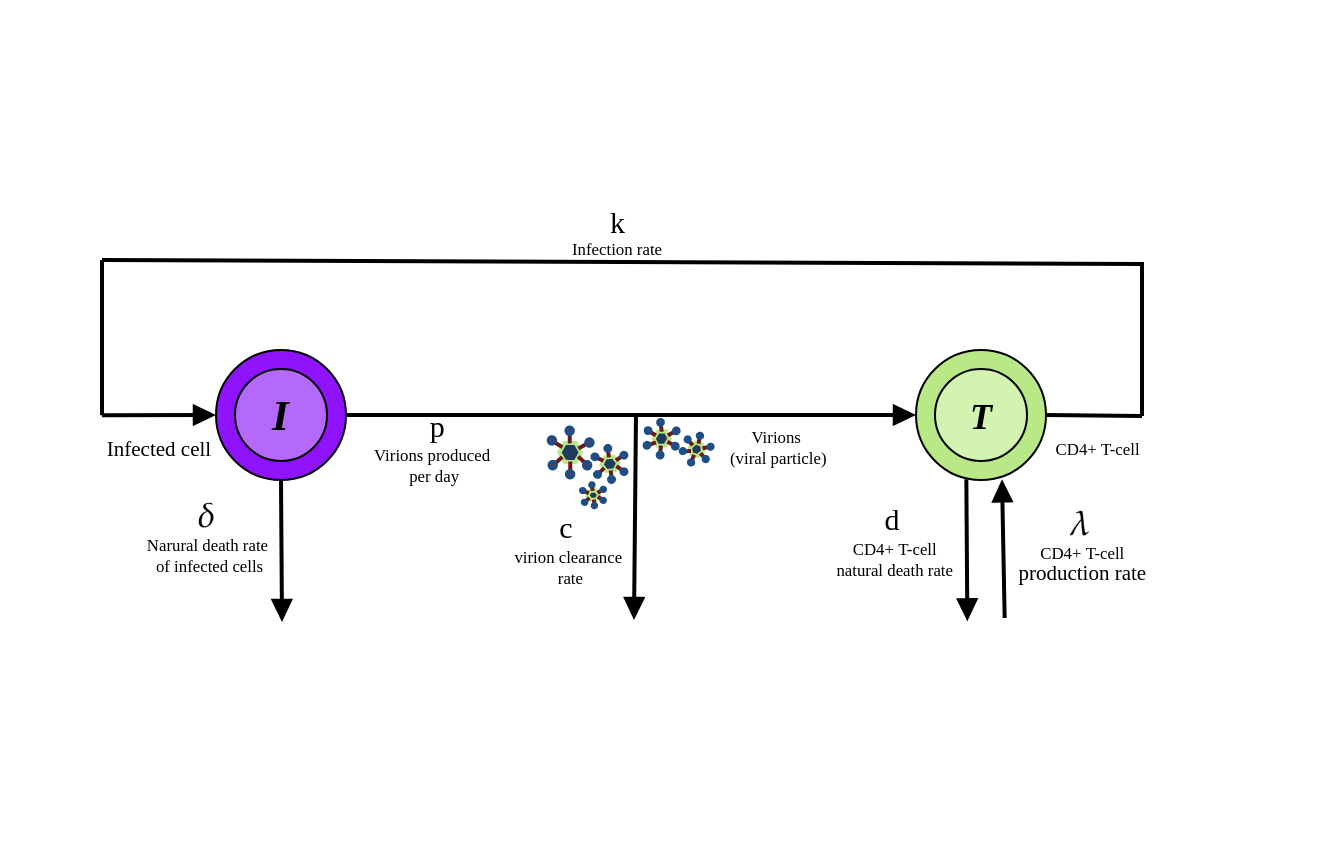
\includegraphics[scale = .2]{Images/TIV.png}
      \caption{TIV flow chart}
      \label{fig:1}
\end{figure}

Variables $T$, $I$, and $V$ have already been established as uninfected CD4$^{+}$ T-cells, infected CD4$^{+}$ T-cells, and the virus, respectively. New CD4$^{+}$ T-cells are created by the body, by, for example, the thymus, at rate $\lambda$ that each have a life span of $1/d$, making the natural death rate of CD4$^{+}$ T-cells: $d$. Target cells $T$ become infected by the virus $V$ at rate $k$; therefore $kVT$ is the rate of infection. Infected cells, $I$, naturally die at rate $\delta$. New virions are produced by infected cells $I$ at rate $p$ and are removed from the body at clearance rate $c$ per virion. Further examination of this model can be found \href{https://doi.org/10.1137/S0036144598335107}{here}.
 
\subsection{Improving model accuracy}
While simpler models are significantly easier to visualize and understand, they often make assumptions and simplifications. For example, Perelson et al. (1999) \cite{perelson1999} adds another operation to the equation $\frac{dT}{dt}$ to account for cell proliferation (cell proliferation is when a cell grows and then divides itself, producing multiple new cells). This equation looks like the following \cite{perelson1999}: 

\begin{equation}\label{eq. (2)}
    \ \frac{dT}{dt} = s + p T \bigg(1 - \frac{T}{T_{max}}\bigg) - d T - k V T
\end{equation}

Where $s$ takes the place of $\lambda$ from \ref{eq. (1)} as the rate of CD4$^{+}$ T-cell production, $p$ is the maximum proliferation rate, and $T_{max}$ is the population density of T-cells at which cell proliferation turns off. For the purposes of the basic TIV model, accounting for cell proliferation wasn't strictly necessary. However, not including it does alter the results and potential accuracy of the model. Often, these simplifications are made due to their not being entirely relevant to the model at hand and their not being presence will not change the overall trend of the graph and are therefore, not necessary. 

When CD4$^{+}$ T-cells are attacked, they send a signal to other types of T-cells that then triggers an immune response. CD8$^{+}$ T-cells are responsible for responding to this attack. When a signal has been received, CD8$^{+}$ T-cells are then considered 'activated'. Activated CD8$^{+}$ T-cells become Cytotoxic T Lymphocytes (CTL) that secrete granzymes capable of killing HIV \cite{CD8}. This process is not covered by typical HIV models, despite its importance to understanding the immune response. The addition of a CD8$^{+}$ T-cell and a CTL compartment enables one to evaluate the interactions between activated CD8$^{+}$ T-cells and other parts of the model, most importantly, with the viral load. 

The final model, outlined below, includes the dynamics of the CD8$^{+}$ and CTL T-cells, in an attempt to demonstrate the immune response. There are two additional compartments-- ($Z$ and $Z_{a}$) that represent such cells. Like in the basic TIV model, $T$ is the uninfected CD4$^{+}$ T-cells, $I$ is the infected CD4$^{+}$ T-cells, and $V$ is the viral load. $Z$ and $Z_{a}$ are CD8$^{+}$ T-cells and Activated CD8$^{+}$ T-cells (CTL's) respectively. The model is as follows \cite{OCM}:

\begin{equation}\label{eq. (3)}
    \begin{split} 
        &    \frac{dT}{dt} = \lambda_T - \mu_T T - \beta_T T V \\
        &    \frac{dI}{dt} = \beta_T T V - \mu_I I- p_I I Z_a \\
        &    \frac{dV}{dt} = k_V \mu_I I - \mu_V V - p_V V Z_a \\
        &    \frac{dZ}{dt} = \lambda_Z - \mu_Z Z - \beta_Z Z V \\
        &    \frac{dZ_a}{dt} = \beta_Z Z V - \mu_Z Z_a\\
    \end{split}
\end{equation} 

%diagram 2
\begin{figure}[thpb]
      \centering
      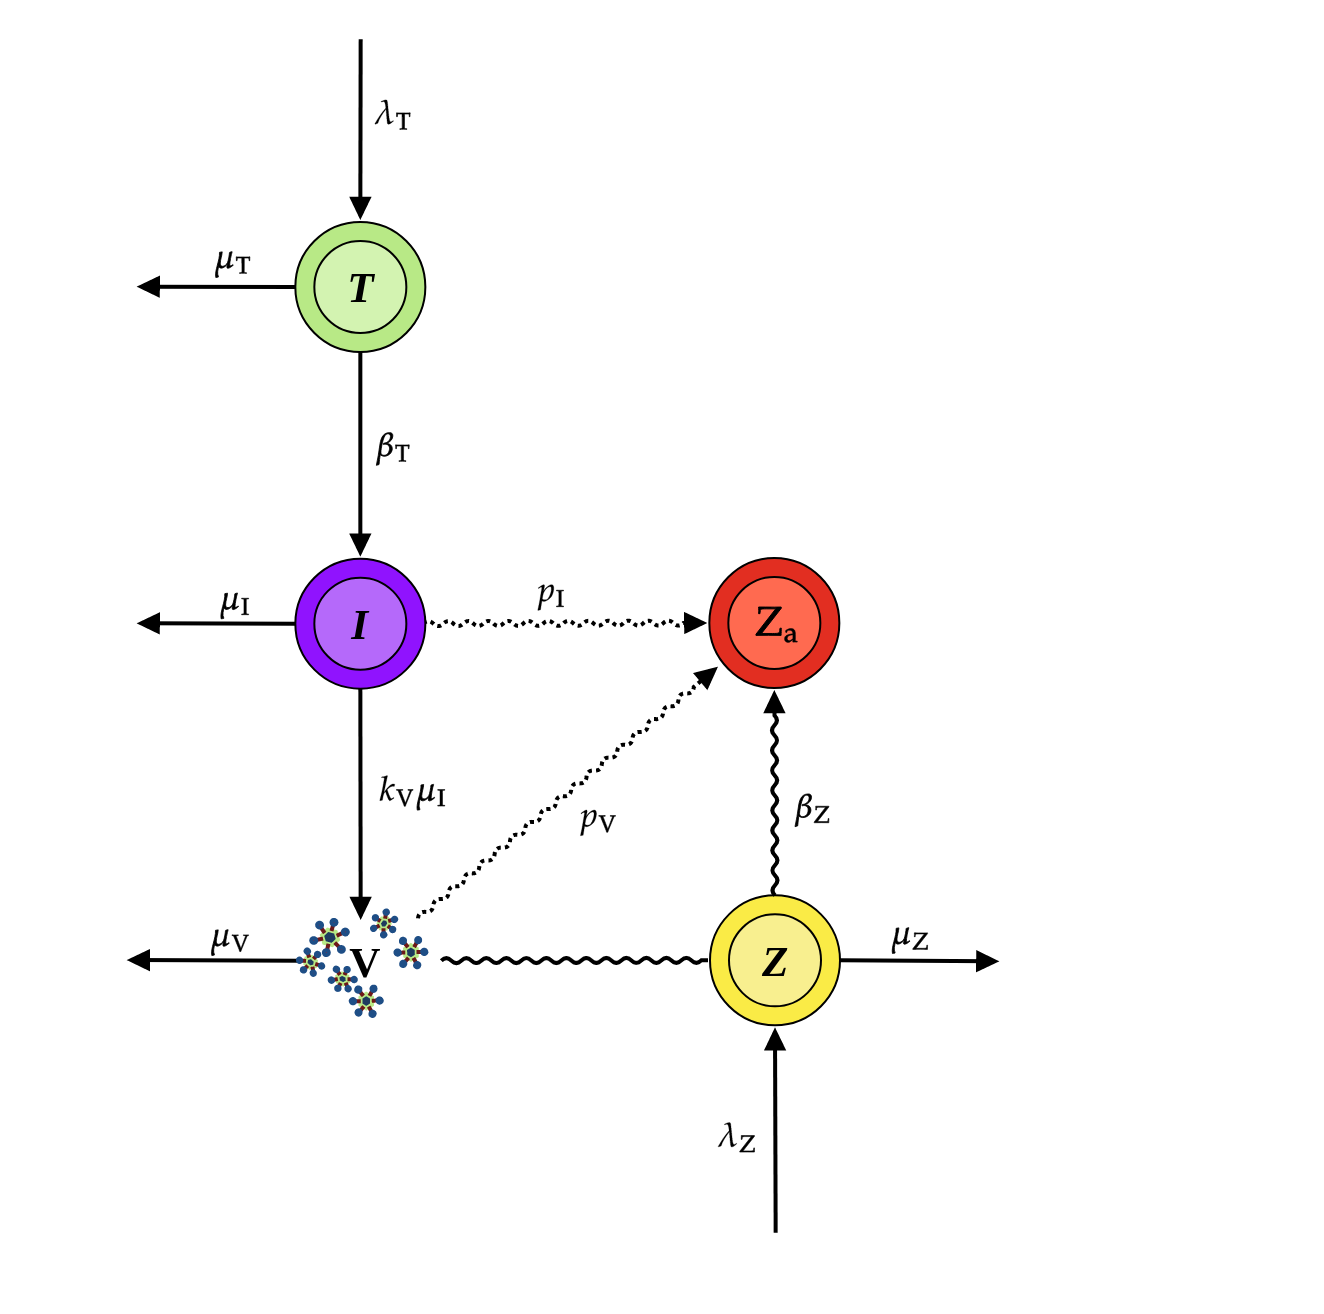
\includegraphics[scale = .2]{Images/TIVZZa.png}
      \caption{Adding immune response to the TIV system}
      \label{fig:2}
\end{figure}

Where $\lambda_{T}$ is the CD4$^{+}$ T-cell production rate and $\lambda_{Z}$ is the production rate of CD8$^{+}$ T-cells. $\mu_{T}$ is the natural death rate of uninfected cells, $\mu_{I}$ is the natural death rate of infected cells, $\mu_{V}$ is the natural death rate of HIV virions, and $\mu_Z$ is the natural death rate for CD8$^{+}$ T-cells (activated or not). $k_{V}$ is the average number of virions produced per infected cell. $p_{I}$ and $p_{V}$ are the destruction and clearance rate of infected cells $I$ and virions $V$. $\beta_{V}$ is the rate at which CD4$^{+}$ T-cells become infected and $\beta_{Z}$ is the rate at which CD8$^{+}$ T-cells become activated (see \ref{table (2)}). 

% Table 1
\begin{table*}[h]
    \caption{Initial Values}
    \begin{center}
    \begin{tabular}{|c|c|p{5cm}|c|}
        \hline
        \thead{Variable} & \thead{Value} & \thead{Definition} & \thead{Source} \\
        \hline% \hline
        $T$ & 1000  mm$^{-3}$ & Number of uninfected CD4$^{+}$T-cells & \cite{OCM}\\
        $I$ & 0 mm$^{-3}$ & Number of infected CD4$^{+}$T-cells & \cite{OCM}\\
        $V$ & 0.001 mm$^{-3}$ & Free HIV virions & \cite{OCM}\\
        $Z$ & 500 mm$^{-3}$ & HIV specific CD8$^{+}$T-cells & \cite{OCM}\\
        $Z_{a}$ & 0 mm$^{-3}$ & Activated CD8$^{+}$T-cells & \cite{OCM} \\
        \hline
    \end{tabular}
    \label{table (1)}
\end{center}
\end{table*}

\begin{table*}[ht!]
    \caption{Parameters}
    \begin{center}
    \begin{tabular}{|c|c|c|c|}
        \hline
        \thead{Symbol} & \thead{{Value}} & \thead{Definition} & \thead{Source}\\
        \hline %\hline
        $\mu_{T}$ & 0.02 day$^{-1}$ & Natural death rate of uninfected CD4$^{+}$T-cells & \cite{OCM}\\
        $\mu_{I}$ & 0.24 day$^{-1}$ & Natural death rate of infected CD4$^{+}$T-cells & \cite{OCM} \\
        $\mu_{V}$ & 2.4 day$^{-1}$ & Natural death rate of the virus & \cite{OCM}\\
        $\mu_{Z}$ & 0.04 day$^{-1}$ & Natural death rate of CD8$^{+}$T-cells & \cite{OCM} \\
        $k_{V}$ & 360 & Average number of virions produced per infected cell & \cite{OCM} \\
        $\beta_{Z}$ & $5 \times 10^{-6}$ mm$^{3}$ day$^{-1}$ & Rate at which CD8$^{+}$T-cells are activated & \cite{OCM}\\
        $\beta_{V}$ & $2.4 \times 10^{-5}$ mm$^{3}$ day$^{-1}$ & Rate at which CD4$^{+}$T-cells are infected & \cite{OCM}\\
        $p_{I}$ & 0.02 mm$^{3}$ day$^{-1}$ & Rate at which infected CD4$^{+}$T-cells are destroyed & \cite{OCM}\\
        $p_{V}$ & 0.02 mm$^{3}$ day$^{-1}$ & Rate at which viruses and virions are destroyed & \cite{OCM}\\
        $\lambda_{T}$ & 20 mm$^{3}$ day$^{-1}$ & Rate at which CD4$^{+}$T-cells are produced by the body & \cite{OCM}\\
        $\lambda_{Z}$ & 20 mm$^{3}$ day$^{-1}$ & Rate at which CD8$^{+}$T-cells are produced by the body & \cite{OCM}\\
        \hline
    \end{tabular}
    \label{table (2)}
\end{center}
\end{table*}

\begin{figure}[thpb]       
      \centering
      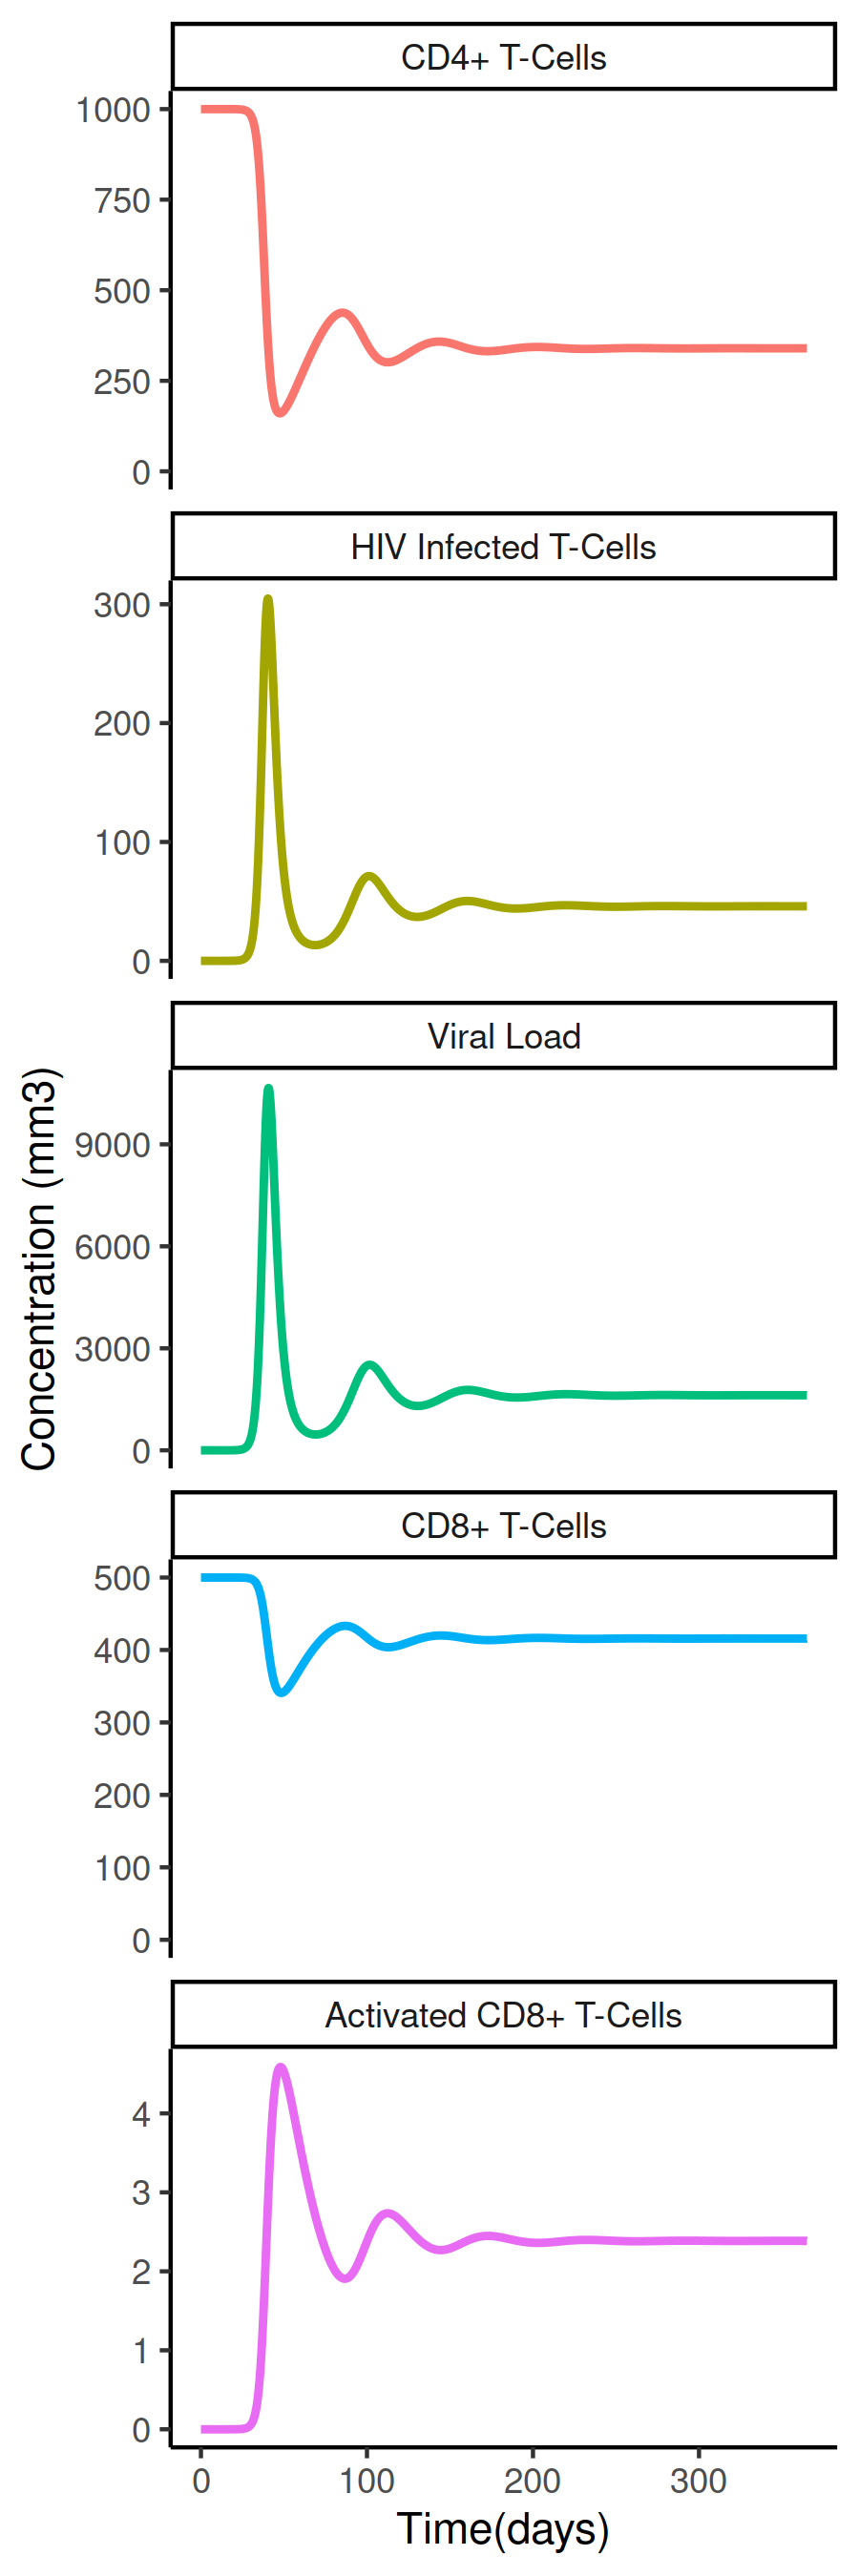
\includegraphics[scale = .5]{Images/result_ocm_1col.png}
      \caption{Modeling the within-host dynamics of HIV with attention to immune response.}
      \label{figure 3}
\end{figure}

%%%%%% ASK ABOUT PLACEMENT OF TABLE 1 AND FIGURE 1
Figure \ref{figure 3} conveys the numerical solution to equation \ref{eq. (3)} using the parameters outlined in tables \ref{table (1)} and \ref{table (2)}. The model was solved using the \texttt{ODE} solver from the R package \texttt{deSolve} using the initial values in table \ref{table (1)}. The model demonstrates a sharp increase in the number of infected cells and viral load within the first 50 days of infection. The increase in infected cells and viral load is confirmed by a sharp decrease in CD4$^{+}$ T-cells. A decrease in CD8$^{+}$ T-cells occurs at the same time; an increase in CTL's (activated CD8$^{+}$ T-cells) is also seen. This lines up with the initial stage of HIV-1 infection: Acute Infection. By day 200 the model has reached steady state, marking the beginning Clinical Latency. 

This model demonstrates the behavior of the immune system inside an HIV infected patient. It allows for the analysis of the body's defense mechanisms in addition to the typical 3 compartment model (TIV). Figure \ref{figure 3} demonstrates peaks (or troughs) for all 5 compartments occurring at the same time, clearly shown by the shared, albeit inverted or upright depending on the graph, shape and timing of each value. The increases, or decreases, in each compartment is proportional to the changes in its related compartment. This model has not yet been adapted for long term infection and does not account for the transition from late stage 2 HIV to AIDS. An important part of HIV modeling is including drug therapies, this will be examined in the next section. 

\section{Adding Antiretroviral Therapy: Reverse Transcriptase Inhibitors}

\subsection{Antiretroviral Therapy}
3 enzymes vital to the productive infection of a cell with HIV, were quickly identified as the reverse transcriptase, integrase, and protease enzymes \cite{LookBack}. Reverse transcriptase takes viral RNA and turns it into DNA, so that viral DNA can be joined with the cell's DNA, this is step 4 in section \ref{Viral Life Cycle} \cite{HIVlifeCycle}. The integrase enzyme completes the second half of this process, by, as the name suggests, integrating the viral DNA into the cell's (step 5, \ref{Viral Life Cycle}) \cite{HIVlifeCycle}. The protease enzyme has a different job. As the last step in the process, protease finishes the maturation of an HIV virion that has burst from the host cell \cite{HIVlifeCycle}. The identification of these three enzymes have provided opportunities for targeted drug therapies.

In 1987, the first drug was approved to treat HIV \cite{LookBack}. AZT (full name azidothymidine), originally used to treat cancer, is a reverse transcriptase inhibitor (RTI). It's success was short lived as drug resistant variants of HIV took over. Since then, combination antiretroviral therapies have become the standard of HIV care. There are 5 classes of antiretroviral therapies (ART's) used to treat HIV, table \ref{table (3)} outlines the purpose of each drug class. Combination antiretrovirals (cARV's) typically include 3 or more drugs from more than one class, in an attempt to overcome HIV's adaptive and drug resistant nature \cite{ART}. \\

\begin{table*}
    \caption{Antiretroviral Classes}
    \begin{center}
    \begin{tabular}{|c|p{7cm}|c|c|}
        \hline
        \thead{Drug Class} & \thead{{Purpose}} & \thead{Step Blocked} & \thead{Source}\\
        \hline 
        Reverse Transcriptase Inhibitors$^{*}$ & Prevents viral RNA from being converted to DNA, prevents virus from productively infecting the cell & 4 & \cite{ART}\\
        Protease Inhibitors$^{**}$ & Prevents new virions from maturing, meaning non-infectious viral particles are produced & 10 & \cite{ART} \\
        Integrase Inhibitors & Blocks integration of HIV DNA with cell DNA & 5 & \cite{ART}\\
        Entry Inhibitors & Stops HIV from binding to, and then entering, a cell & 2 & \cite{ART} \\
        Pharmacokinetic (PK) Inhibitors & Prevents drug breakdown allowing another drug to remain in the body for longer boosting another drugs effectiveness & N/A & \cite{ART} \\
        \hline
        \multicolumn{4}{l}{\footnotesize{$^{*}$ There are two sub-classes of RTI's: Nucleoside Reverse Transcriptase Inhibitors (NRTI's) and Non-Nucleoside Reverse Transcriptase}}\\
        \multicolumn{4}{l}{\footnotesize{\hspace{3.5mm}Inhibitors (NNRTI's). They both produce the same result, but interfere with reverse transcriptase in a different way.}}\\
        \multicolumn{4}{l}{\footnotesize{$^{**}$ Protease inhibitors have \textit{no} effect on already existing viral particles.}}
    \end{tabular}
    \label{table (3)}

\end{center}
\end{table*} 


\subsection{Adding a Reverse Transcriptase Inhibitor}
To make equation \ref{eq. (3)} more applicable to HIV research, a new model has been adapted to demonstrate the effects of an ART. The next section outlines a model in which a reverse transcriptase inhibitor is included.

RTI's effectively inhibit the production of new virions and will therefore effect \(\beta_V T V\) (the number of productively infected cells). Based on the adaptation of Perelson et al.'s basic model, the effectiveness of Emtricitabine (an NRTI) was added to equation \ref{eq. (3)}. Accounting for the use of Emtricitabine, equation \ref{eq. (3)} now looks like the following: 

\begin{equation}
    \begin{split}
        &   \frac{dT}{dt} = \lambda_T - \mu_T X - N_{RTI} \beta_V T V \\
        &   \frac{dI}{dt} = N_{RTI} \beta_V T V - \mu_I - p_I I Z_a \\
        &   \frac{dV}{dt} = k_V \mu_I I - \mu_V V - p_V V Z_a \\
        &   \frac{dZ}{dt} = \lambda_Z - \mu_Z Z - \beta_Z Z V \\
        &   \frac{dZ_a}{dt} = \beta_Z Z V - \mu_Z Z_a \\
    \end{split}
\end{equation}

Where $N_{RTI}$ represents the effectiveness of the RTI. The effectiveness of Emtricitabine was calculated as a range of minimum and maximum efficacy using the values outlined in table \ref{table (3)}. 

%table 3
\begin{table*}
\caption{Emtricitabine Efficacy Parameters}
\begin{center}
    \begin{tabular}{|c|c|c|c|}
        \hline
        \thead{Symbol} & \thead{Value} & \thead{Definition} & \thead{Source}\\
        \hline 
        $C_{min}$ & 0.064 $\mu$g/mL & Minimum concentration of Emtricitabine at steady state & \cite{Cmin/max} \\
        $C_{max}$ & 1.77 $\mu$g/mL & Maximum concentration of Emtricitabine at steady state & \cite{Cmin/max} \\
        $EC_{50_{min}}$ & 0.0013 $\mu$M & Minimum $EC_{50}$ of Emtricitabine & \cite{EC50} \\
        $EC_{50_{max}}$ & 0.64 $\mu$M & Maximum $EC_{50}$ of Emtricitabine & \cite{EC50} \\
        $n$ & 1 & Hill Coefficient of NRTI's & \cite{hillCoefficient}\\
        \hline
    \end{tabular}
\end{center}
\end{table*}

Drug efficacy was calculated using these equations adapted from \cite{drugEfficacy}:

\begin{equation}
    \begin{split}
        & N_{RTI_{min}} = \frac{C_{min}^n}{C_{min}^n + EC_{50_{min}}^n} \\
        & N_{RTI_{max}} = \frac{C_{max}^n}{C_{max}^n + EC_{50_{max}}^n}
    \end{split}
\end{equation}

A drug's $EC_{50}$ value is the concentration [of the drug] that will produce 50\% of the maximal response. It is the industry standard way to compare drug potency's (high $EC_{50}$ low potency, low $EC_{50}$ high potency). $C$ is denoted as the steady state plasma concentration; therefore $C_{max}$ is the peak (maximal) concentration at steady state and $C_{min}$ is the minimum concentration at steady state. $n$ is the Hill Coefficient, a way of measuring drug "cooperation". \\

The new model:
\begin{figure}[thpb]
      \centering
      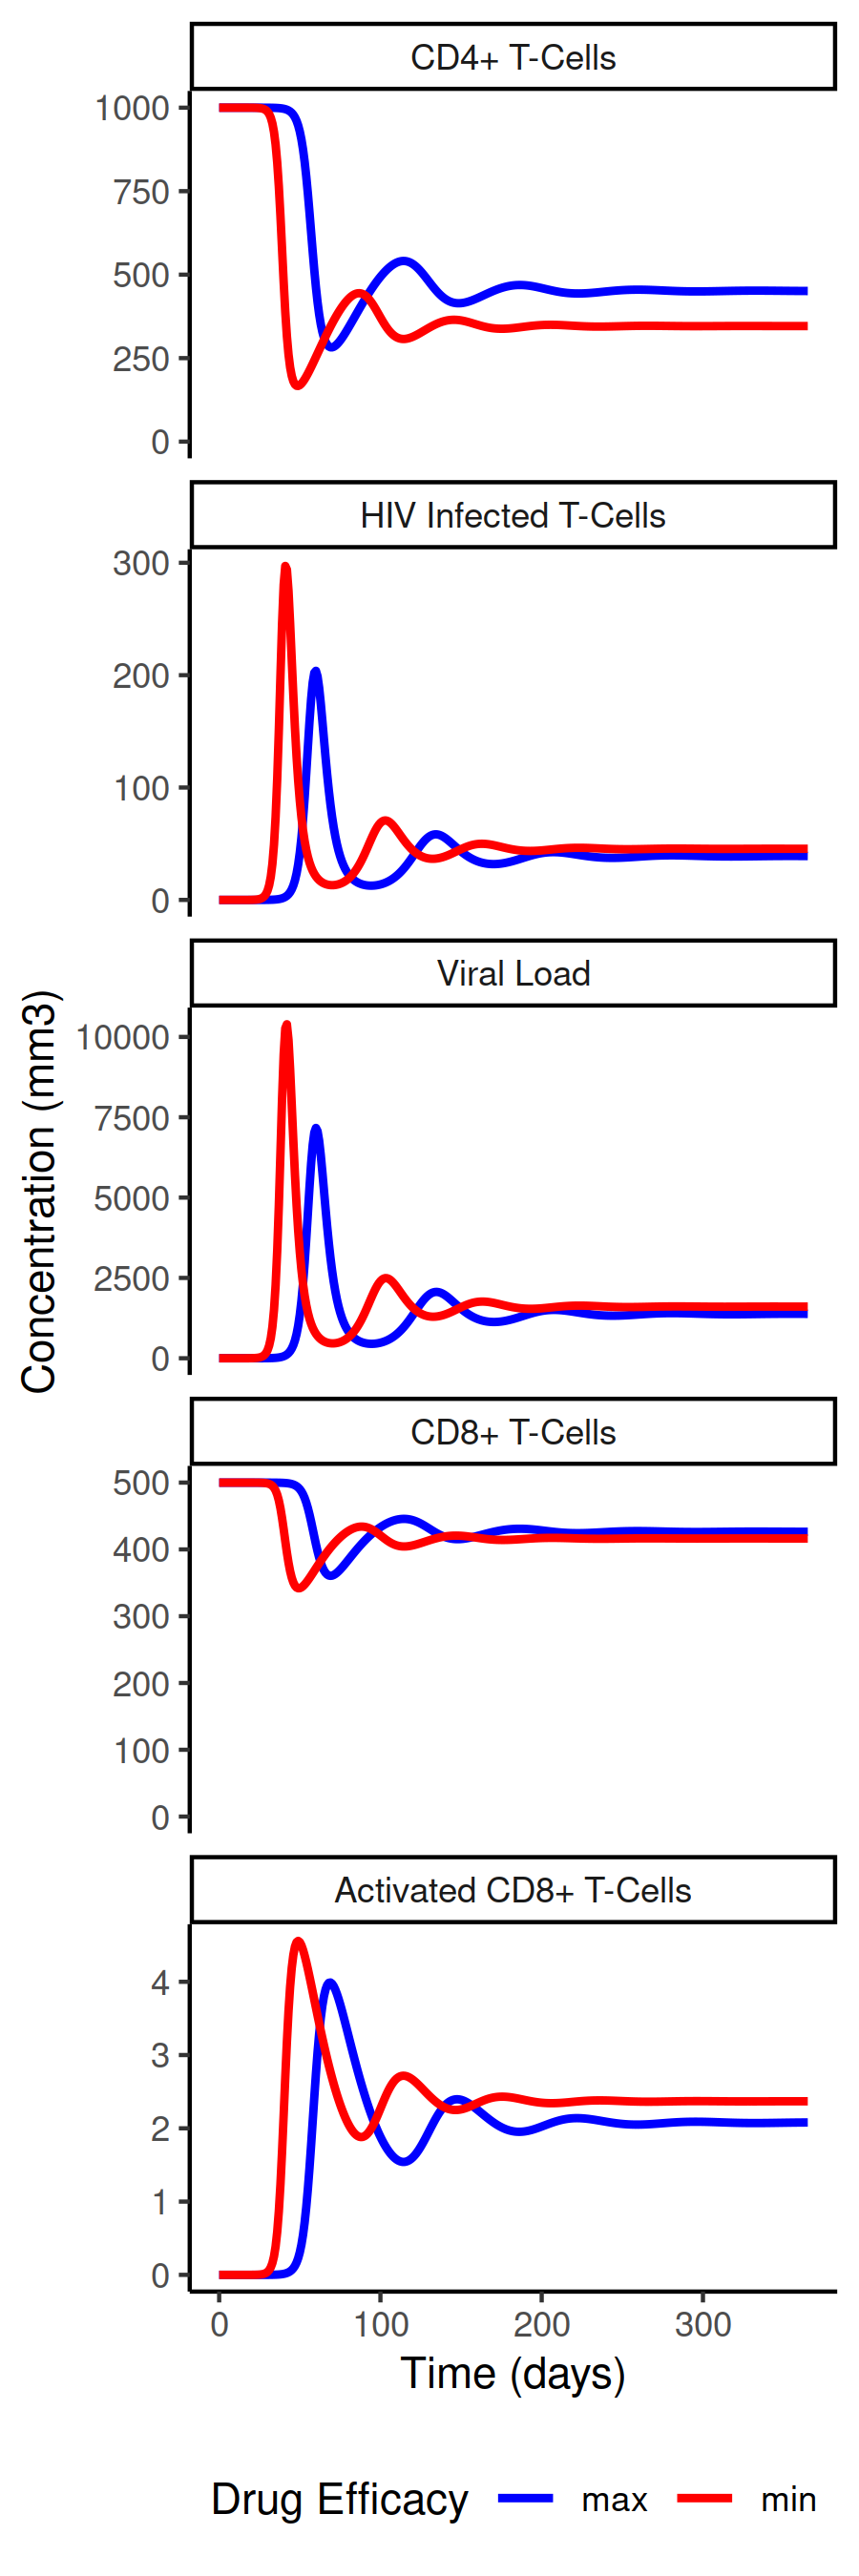
\includegraphics[scale = 0.72]{Images/result_ocm_rti_1col.png}
      \caption{Adding Emtricitabine to equation \ref{eq. (3)}, to demonstrate the minimum and maximum drug effect on the immune system and viral load.}
      \label{fig:4}
\end{figure}

The minimum efficacy of Emtricitabine is quite close to zero, making the minimum efficacy values (red) quite close to the original model.  With this in mind, interpreting the effects Emtricitabine on the immune system and viral load becomes quite straight forward. The peaks and troughs of $N_{max}$ are of lower values than that of $N_{min}$. They also occur at later dates, roughly 25 days, than their minimal counterparts. What this shows is that not only does the drug decrease the number of infected cells and the subsequent virions, thereby increasing the number of uninfected CD4$^{+}$ T-cells, but that it also temporarily halts the progression of HIV. By extending the period of time before Acute and Chronic infection, the development of AIDS is prolonged, for some that can be more than 30 years \cite{cARVtimeline}. 

\section{CONCLUSION}
The complexities of HIV are hard to describe in a single model. What this paper attempts to do is not to cover every aspect of the disease, but rather provide a foundational understanding of HIV and how it interacts with the immune system. The dynamics of an antiretroviral drug, Emtricitabine, were also explored. 

It is important to note that the models shown do not represent the total population of HIV positive persons, but when it comes to mathematical modeling, it never will. Modeling aims to show a generalized over view of, often times, very complex systems that can be hard to track. In this case, being able to model, for example, CD4$^{+}$ T-cells and viral load before and after treatment, enables care providers, policy makers, and patients themselves to understand what is happening inside the body without the need for exhausting tests, cell counts, and re-tests. The advances made in HIV modeling have enabled researchers to extend the reach of the model beyond HIV, using the technology and mathematics to model other viruses such as Hepatitis B \& C, and CMV \cite{TIVdiagram}.

This model is the basis of a future resource for people impacted by HIV. As discussed in section 1, stigma surrounding HIV is rampant. Although conversation surrounding STD's as a whole is becoming more common, many still feel isolated and can be hesitant to reach out for testing, treatment, and support. We hope to create an online resource available to anyone impacted by HIV, so as to provide them with greater education and understanding of HIV/AIDS, treatment options, and other, external supports and care. Fighting the stigma associated with HIV is an up hill battle. Hopefully with greater health initiatives and access to accurate, scientific information we can begin to combat this. Globally, HIV infection rates have declined by 38\% since 2010 and 76\% of people living with HIV are taking antiretroviral medications \cite{UNaids}. With increased access to education and treatment, we can continue this trend across the globe, simultaneously combating the stigma of HIV and the virus itself. 

\addtolength{\textheight}{-12cm}   

\section*{ACKNOWLEDGMENTS}

This work was done in collaboration with Valeria Gracia Olvera and made possible by the Institute for Computing in Research. 

\printbibliography

\end{document}
